\usepackage{xcolor}
\usepackage{afterpage}
\usepackage{pifont,mdframed}
\usepackage[bottom]{footmisc}
\usepackage{minted}

\createsection{\Grader}{Grader di prova}

\newcommand{\inputfile}{\texttt{stdin}}
\newcommand{\outputfile}{\texttt{stdout}}
\makeatletter
\renewcommand{\this@inputfilename}{\texttt{stdin}}
\renewcommand{\this@outputfilename}{\texttt{stdout}}
\makeatother

% % % % % % % % % % % % % % % % % % % % % % % % % % % % % % % % % % % % % % % % % % %
% % % % % % % % % % % % % % % % % % % % % % % % % % % % % % % % % % % % % % % % % % %

Nel cuore della misteriosa isola di Zeria, gli avventurieri trovano un antico tempio protetto da un complicato
meccanismo matematico.

\begin{figure}[h]
    \centering
    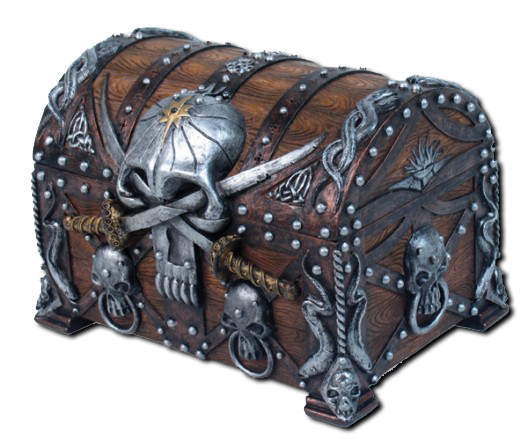
\includegraphics[width=0.5\textwidth]{chest.png}
    \caption{Il tesoro del tempio di Zeria.}
\end{figure}

L'enigma è il seguente:

"\textit{Dato un numero intero $N$, qual è il numero di zeri finali di $N$ fattoriale?}"

Riesci a risolvere l'enigma?
\begin{warning}
    $N$ fattoriale (scritto anche come $N!$) è equivalente a $1 \cdot 2 \dots N$.
\end{warning}




\Implementation

Dovrai sottoporre un unico file, con estensione \texttt{.cpp}.

\begin{warning}
    Tra gli allegati a questo task troverai un template \texttt{zeria.cpp} con un esempio di implementazione.
\end{warning}

Il file di input è composto da $1$ riga:
\begin{itemize}
    \item Riga 1: l'intero $N$.
\end{itemize}

Il file di output è composto da $1$ riga:
\begin{itemize}
    \item Riga 1: la risposta al problema.
\end{itemize}

% % % % % % % % % % % % % % % % % % % % % % % % % % % % % % % % % % % % % % % % % % %
% % % % % % % % % % % % % % % % % % % % % % % % % % % % % % % % % % % % % % % % % % %

\Constraints

\begin{itemize}[nolistsep, itemsep=2mm]
    \item $1 \le N \le 10^{18}$.
\end{itemize}

% % % % % % % % % % % % % % % % % % % % % % % % % % % % % % % % % % % % % % % % % % %
% % % % % % % % % % % % % % % % % % % % % % % % % % % % % % % % % % % % % % % % % % %

\Scoring

Il tuo programma verrà testato su diversi test case raggruppati in subtask.
Per ottenere il punteggio relativo ad un subtask,
è necessario risolvere correttamente tutti i test che lo compongono.

\begin{itemize}[nolistsep,itemsep=2mm]
    \item \subtask Casi d'esempio.
    \item \subtask $N  \le 20$
    \item \subtask $N \le 1\:000\:000$
    \item \subtask Nessuna limitazione aggiuntiva.
\end{itemize}

% % % % % % % % % % % % % % % % % % % % % % % % % % % % % % % % % % % % % % % % % % %
% % % % % % % % % % % % % % % % % % % % % % % % % % % % % % % % % % % % % % % % % % %

\Examples

\begin{example}
    \exmpfile{zeria.input0.txt}{zeria.output0.txt}%
\end{example}

% % % % % % % % % % % % % % % % % % % % % % % % % % % % % % % % % % % % % % % % % % %
% % % % % % % % % % % % % % % % % % % % % % % % % % % % % % % % % % % % % % % % % % %

\Explanation

Nel caso d'esempio, $5! = 120$, che termina con $1$ zero.
